\documentclass{ximera}
\graphicspath{
{./}
{volumes/}
{arclengths/}
{centroids/}
{techniques/}
{applications/}
{series/}
{powerseries/}
{odes/}
{lessons/}
}
\usepackage{booktabs}

\newcommand{\bigmath}[1]{$\displaystyle #1$}
\newcommand{\choicebreak}{}
\newenvironment{type}{}{}
\newenvironment{notes}{}{}
\newenvironment{keywords}{}{}
\newcommand{\offline}{}
\newenvironment{comments}{\begin{feedback}}{\end{feedback}}
\newenvironment{multiplechoice}{\begin{multipleChoice}}{\end{multipleChoice}}
\title{Applications of ODEs}
%%%%%\author{Philip T. Gressman}

\begin{document}
\begin{abstract}
We study some sample applications of ODEs.
\end{abstract}
\maketitle

\section*{(Videos) Calculus: Single Variable}
\youtube{54HrJmeON24}
\youtube{xZ3CxLxljLA}


\section*{Examples}

\begin{example}
Newton's law of cooling states that the rate of change of the temperature of an object is proportional to the \textit{difference} between the object's temperature and the ambient temperature.
For example, if the ambient temperature is $20$ degrees Celsius, then
\[ \frac{dT}{dt} = -k \left( T(t) - \answer{20} \right). \]
(Here $k$ is a positive number is called the \textit{heat transfer coefficient}; it depends on the physical properties of the object and the surrounding environment).
\begin{itemize}
\item The equation is linear:
\[ \frac{dT}{dt} + k T = \answer{20} k. \]
\item In this case, $P(t) = \answer{k}$ and the integrating factor is $\answer{e^{k t}}$ (since $k$ is a constant with respect to $t$).  The general solution is
\[ T(t) = \answer{20} + C \answer{e^{-k t}}. \]
\item If we subtract ambient temperature from both sides, this tells us that the temperature difference decays exponentially at some rate determined by the unknown constant $k$.
\item We can generally solve for $k$ if we have enough information.  For example, if $T(0) = 100$, then $C = \answer{80}$.  If we also know that $T(10) = 60$, then $C e^{-10 k} = 40$ (because $40$ is the difference of $60$ and $20$), which means $k = \answer{(\ln 2)/10}$. Another way of understanding this exponential decay is to observe that the temperature difference for this particular object will be cut in half every ten minutes.
\item Now that we know $k$, we can compute $T(t)$ for all time. For example, $T(20) = \answer{40}$, which we could see by plugging in directly to the solution or by merely observing that the temperature difference will be cut in half $\answer{2}$ times in the course of 20 minutes.
\end{itemize}
\end{example}


\begin{example}
For the family of curves in the plane given by 
\[ x^4 + y^2 = C \]
(illustrated by the purple oval-shaped curves in the image below), 
find a formula for the orthogonal trajectories (shown in red).
\begin{center}
\begin{image}
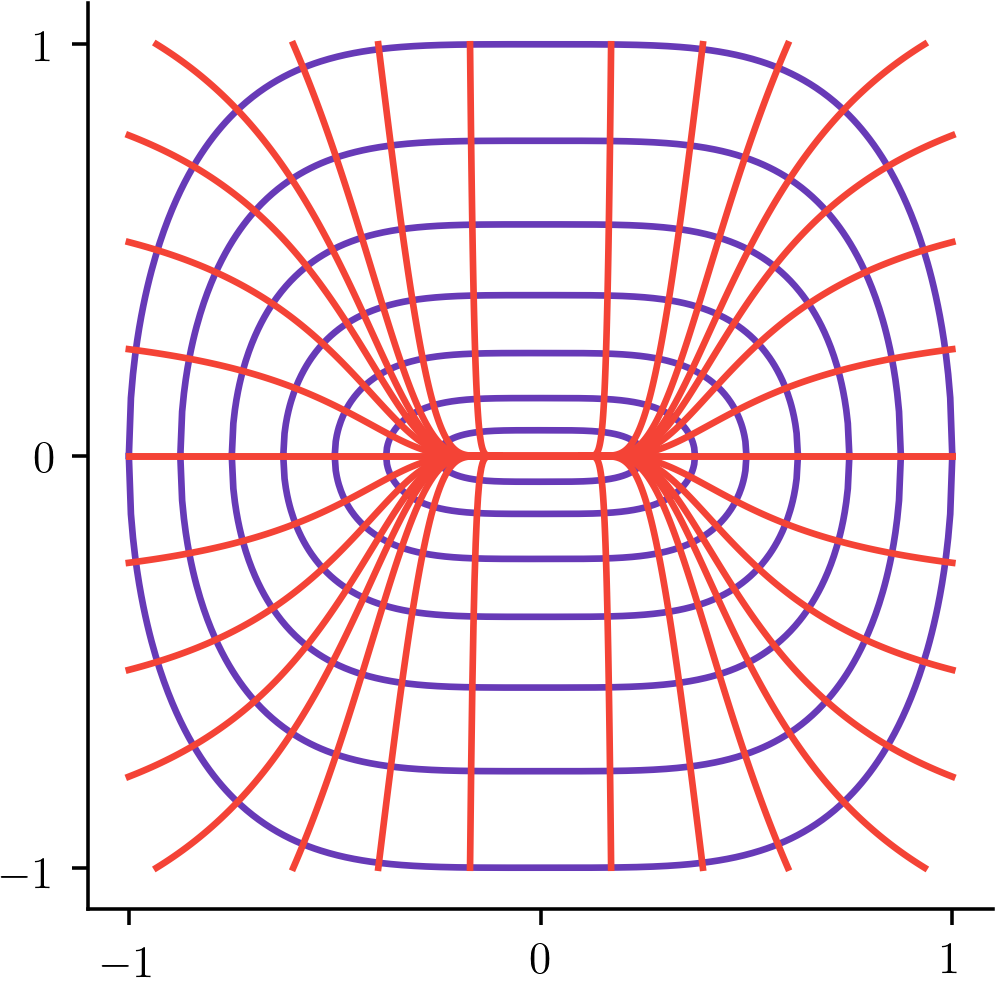
\includegraphics[width=4in]{images/orthoX01.png}
\end{image}
\end{center}
\begin{itemize}
\item The first step is to find a first-order ODE that is satisfied by the family. This involves differentiating with respect to $x$. We get
\[ 4 x^3 + 2y y' = 0, \ \text{ meaning } y' = \answer{-\frac{2x^3}{y}}. \]
\item If $m$ and $m'$ are slopes of orthogonal lines, then $m m' = -1$. So the orthogonal trajectories satisfy an ODE similar to the one above except that the formula for $y'$ is replaced by its negative reciprocal, i.e.,
\[ y' = \answer{\frac{y}{2x^3}}. \]
\item This is a separable ODE. It separates to
\[ \frac{dy}{\answer{y}} = \frac{1}{2} \frac{dx}{\answer{x^3}}. \]
Integrating both sides gives
\[ \ln |y| = - \frac{1}{4} x^{-2} + C. \]
If we exponentiate both sides and reexpress the arbitrary constant, we get
\[ y = C \answer{e^{-\frac{1}{4x^2}}} \]
\end{itemize}
\end{example}


\begin{example}
For the family of curves in the plane given by 
\[ y = \frac{1}{C + x^2} \]
(shown in purple)
find a formula for the orthogonal trajectories (shown in red).
\begin{center}
\begin{image}
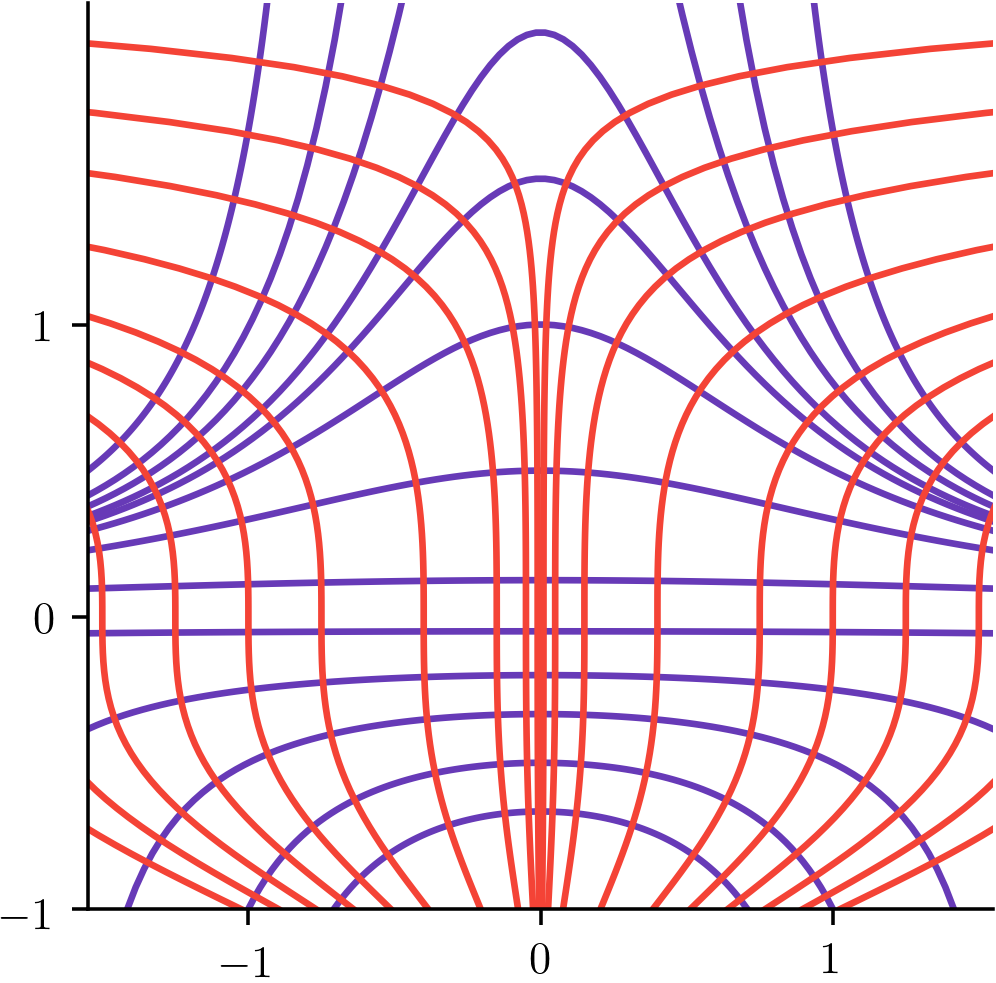
\includegraphics[width=4in]{images/orthoX02.png}
\end{image}
\end{center}
\begin{itemize}
\item We first differentiate with respect to $x$:
\[ y' = \answer{ - \frac{2x}{(x^2+C)^2}}. \]
\item Next we must eliminate $C$ from the equation for $y'$ by using the formula $y = 1/ (x^2+C)$. (For example, solve for $C$ in terms of $x$ and $y$ and then substitute this in to your expression for $y'$.)
\[ y' = \answer{ - 2 x y^2} \]
(your answer here will depend on the variables $x$ and $y$ but should not explicitly depend on $C$).
\item Then we write a new ODE whose slope is the negative reciprocal of the expression we just found:
\[ y' = \answer{\frac{1}{2xy^2}}. \]
This is a separable ODE:
\[ \answer{y^2} dy = \frac{1}{2} \frac{dx}{\answer{x}}. \]
\item Integrate both sides:
\[ \answer{\frac{y^3}{3}} = \frac{1}{2} \answer{\ln |x|} + C. \]
(Don't forget absolute values on logarithms.)
\end{itemize}
\end{example}

\begin{example}
A large 100 liter tank is initially filled with fresh water. At time $t=0$, a technician begins pouring in $2$ liters per minute of sugar water which is at a concentration of 4 grams per liter. At the same time, another technician opens a valve at the bottom of the tank and begins to drain the tank at a rate of $1$ liter per minute. Assuming the whole tank is kept well-mixed at all times, what is the concentration of the liquid in the tank after 100 minutes?
\begin{itemize}
\item It is always easiest to write an ODE for the total amount $A$ of sugar in the tank (in grams). The concentration can be deduced later by dividing amount by volume.
\item The first step is to find the function $V(t)$ for the total volume of solution in the tank.  The rate of fresh solution coming in is $\answer{2}$ liters per minute and the rate going out is $\answer{1}$ liter(s) per minute. So the net flow in of all liquid is $\answer{1}$ liter(s) per minute. This means that at time $t$, $V(t) = \answer{100 + t}$.
\item Fill in the blanks: $R_{\mathrm{in}}$ is the rate of sugar coming in (measured in grams per minute), $F_{\mathrm{out}}$ is the \textit{volume} rate of flow out from the bottom of the tank. Then
\[ \frac{dA}{dt} = R_{\mathrm{in}} - F_{\mathrm{out}} \frac{A(t)}{V(t)} = \answer{8} - \answer{1} \frac{A(t)}{\answer{t+100}}.\]
\item The equation is linear:
\[ \frac{dA}{dt} + \answer{ \frac{1}{100 + t}} A(t) = \answer{8}. \]
\item We compute the integrating factor:
\[ I(t) = e^{\int P(t) dt} = e^{\int \answer{(t+100)^{-1}} dt} = \answer{t+100}. \]
(Note: logarithms don't need absolute values here because $t  > 0$.)
\item After multiplying both sides by $I(t)$, we have
\[ \left( \answer{(t+100)} A(t) \right)' = \answer{8 (t+100)}. \]
\item Integrating both sides gives
\[ (t+100) A(t) = 4 (t+100)^2 + C. \]
At $t = 0$, $A(0)$ is given to be zero, so $C = \answer{-40000}$. The full solution of the initial value problem is then
\[ A(t) = \answer{4 (t + 100) - \frac{40000}{t+100}}. \]
\item $A(100) = \answer{600}$ grams. Furthermore $V(t) = \answer{200}$ liters, so the concentration at time $t = 100$ minutes is $\answer{3}$ grams per liter.
\end{itemize}
\end{example}


\end{document}
